\documentclass[11pt,a4paper]{article}

\usepackage[T1]{fontenc}
\usepackage[utf8]{inputenc}
\usepackage{lmodern}
\usepackage[a4paper,margin=25mm,headheight=15pt]{geometry}
\usepackage{microtype}
\usepackage{graphicx}
\usepackage{booktabs}
\usepackage{tabularx}
\usepackage{array}
\usepackage{longtable}
\usepackage{float}
\usepackage{caption}
\usepackage{xcolor}
\usepackage{enumitem}
\usepackage{hyperref}
\usepackage{url}

\definecolor{benchblue}{HTML}{185FA5}
\definecolor{benchlight}{HTML}{EAF2F8}
\definecolor{benchdark}{HTML}{17324D}
\hypersetup{
  colorlinks=true,
  linkcolor=benchblue,
  citecolor=benchblue,
  urlcolor=benchblue,
  pdftitle={Evaluating Local LLM Pipelines for Ontology Generation},
  pdfauthor={Gu Mingxuan; Chayan Talukder}
}

\pagestyle{plain}

\setlist[itemize]{leftmargin=*,topsep=4pt,itemsep=2pt}
\setlist[enumerate]{leftmargin=*,topsep=4pt,itemsep=2pt}
\captionsetup{font=small,labelfont=bf}
\renewcommand{\arraystretch}{1.15}
\setlength{\emergencystretch}{2em}
\newcommand{\NA}{\textit{NA}}
\newcommand{\code}[1]{\texttt{#1}}

\begin{document}

\begin{center}
  \vspace*{0.5cm}
  {\LARGE\bfseries Evaluating Local LLM Pipelines\\[0.18em]
  for Ontology Generation\par}
  \vspace{0.35cm}
  {\large Bench4KE: Ollama Support, Documentation Completeness,\\
  and Prompt Sensitivity\par}
  \vspace{0.55cm}
  {\large Gu Mingxuan\par}
  {\small\texttt{mingxuan.gu@studio.unibo.it}\par}
  \vspace{0.22cm}
  {\large Chayan Talukder\par}
  {\small\texttt{chayan.talukder@studio.unibo.it}\par}
  \vspace{0.28cm}
  {\normalsize University of Bologna - Master in Artificial Intelligence\par}
  {\normalsize Knowledge Engineering\par}
  \vspace{0.28cm}
  {\normalsize July 2026\par}
\end{center}

\vspace{0.25cm}

\begin{abstract}
This project evaluates three ontology-generation pipelines---the
Ontogenia-labelled Memoryless CQ-by-CQ baseline, Domain-OntoGen, and
NeOn-GPT---using one local Ollama model. The experiment covers 17
ontology-engineering scenarios, 74 source-ordered competency questions (CQs),
and three prompt variants: the recovered baseline P0, serialization-only P1,
and syntax-verification P2. Across 153 tasks, 101 final ontologies were
parseable. Final parse success was 14/51 for the Memoryless baseline, 50/51 for
Domain-OntoGen, and 37/51 for NeOn-GPT. Paired analysis found no
statistically significant parse-success difference among P0, P1, and P2 for
any method. This result does not imply prompt invariance: descriptive
term-Jaccard summaries show substantial ontology-content drift from P0 where
comparisons are available. Documentation completeness and parse robustness
also varied materially by method. The project supplies the mandatory local
model execution path and two new evaluation components.
\end{abstract}

\section{Introduction}

Large language models can turn scenarios and competency questions into candidate
ontologies, but a useful benchmark must evaluate more than whether a final file
exists. This project records prompts, intermediate outputs, parsing results, and
model telemetry to support analysis of generation failures. Bench4KE provides a starting point for
standardized knowledge-engineering evaluation \cite{ciancarini2026bench4ke},
while Ontogenia and related work establish three generation procedures used in
this project \cite{lippolis2024ontogenia,lippolis2025ontology}.

The course brief requires mandatory Ollama support, at least two additional
evaluation components, and testing on the entire executable normalized dataset
with the three methods already connected to Bench4KE. This submission implements
all three requirements.
It compares the methods under one exact local model and adds documentation
completeness and prompt sensitivity analyses.

\section{Related Work}

Recent work has investigated the use of large language models for ontology
engineering and ontology drafting from natural-language requirements.
Ontogenia introduced a metacognitive prompting strategy for ontology generation
with large language models, using competency questions as part of the
ontology-engineering input \cite{lippolis2024ontogenia}. Subsequent work
studied LLM-based OWL ontology drafting from user stories and competency
questions and evaluated prompting techniques such as Memoryless CQbyCQ and
Ontogenia \cite{lippolis2025ontology}. A separate domain-specific study
evaluated DeepSeek and o1-preview on 95 curated CQs from six domains; its
public companion resource supplies the prompt recovered for the
Domain-OntoGen baseline in this project
\cite{lippolis2025domainspecific}. NeOn-GPT represents a related
LLM-powered ontology-learning pipeline grounded in the NeOn methodology and
designed to translate natural-language domain descriptions into Turtle
ontologies \cite{fathallah2024neongpt}. Bench4KE provides an extensible
benchmark-oriented setting for knowledge-engineering automation, with its first
release focused on automatic competency-question generation and with other KE
tasks left as possible extensions \cite{ciancarini2026bench4ke}. The present
work uses three generation methods available in the project baseline:
Ontogenia, Domain-OntoGen, and NeOn-GPT. Its goal is to extend their evaluation
rather than to propose a new ontology-generation method.

Ontology documentation is a separate concern from syntactic validity and
axiomatic structure. An ontology may be parseable while still being difficult
for humans to inspect, maintain, or reuse because its classes and properties
lack labels, comments, definitions, or ontology-level metadata. Tools such as
WIDOCO treat documentation as an explicit ontology-engineering activity by
detecting missing vocabulary metadata and generating human-readable
documentation and diagrams \cite{garijo2017widoco}. However, documentation
support tools do not directly provide a benchmark for measuring the
documentation produced by LLM-based ontology generators. The C2 component of
this project therefore measures the coverage of labels, comments or
definitions, descriptive metadata, and nontrivial documentation literals in
generated ontologies. These metrics measure documentation presence and
coverage; they do not establish the semantic correctness of the annotations or
of the ontology itself.

Prompt robustness has also become an important concern in LLM evaluation.
PromptBench studies the robustness of large language models to adversarial
prompt perturbations, including character-level, word-level, sentence-level,
and semantic-level changes \cite{zhu2023promptbench}. Such sensitivity is
particularly relevant to ontology generation because a response must satisfy
both domain-modeling requirements and a strict serialization grammar.
Nevertheless, the C3 experiment in this project is narrower than general
adversarial or semantic prompt-robustness evaluation. P1 and P2 are append-only
instruction suffixes applied to the recovered P0 prompts. Scenarios,
competency questions, examples, method procedures, call structures, parsing
policies, and generation controls remain fixed. C3 consequently evaluates
instruction-level suffix sensitivity through paired parse-success outcomes and
ontology-term Jaccard overlap; it does not evaluate unrestricted semantic
rephrasing.

The project specification additionally identifies local open-model execution
as a missing benchmark capability. Local execution can reduce dependence on
paid services. The implementation records the runtime version, model tag,
generation controls, prompts, responses, telemetry, parse stages, and repair
behavior. The empirical conclusions remain limited to one quantized Qwen model,
one seed, and one fixed context and output budget, and therefore should not be
generalized to all open models.

In summary, the project brings together three complementary concerns:
LLM-based ontology generation, ontology documentation, and prompt robustness.
Its contribution is an extension of the project benchmark with local Ollama
execution, documentation-completeness metrics, and a narrowly
controlled prompt-sensitivity analysis. It does not claim to solve general
ontology-quality evaluation or broad prompt robustness.

\section{Objectives and Contributions}

The project delivers three benchmark extensions:

\begin{enumerate}
  \item \textbf{C1---native local Ollama execution.}
  The provider records model information, generation controls, requests,
  responses, per-step telemetry, parsing stages, and errors.

  \item \textbf{C2---documentation completeness.}
  The evaluation measures labels, comments or definitions, ontology
  metadata, documentation length, and nontrivial documentation for parseable
  generated ontologies.

  \item \textbf{C3---prompt sensitivity.}
  P0/P1/P2 variants are compared through paired parse-success tests and
  ontology-term Jaccard overlap under a prespecified statistical policy.
\end{enumerate}

All experimental generation used the local Ollama model described below.

\section{Dataset Construction}

The normalized full-generation dataset contains 17 scenarios and 74 executable
CQs. The source workbook contains 112 nonempty CQ rows. Thirty-eight rows are
retained in audit records but excluded from executable generation because they
lack reliable StoryID or scenario linkage. The pipeline does not infer or
fuzzily reconstruct missing links.

Scenarios, user stories, and CQs were recovered from the source workbook through
explicit source relationships. CQ wording and source order are preserved. Every
managed data file was validated with its expected parser and encoding, and the
normalized JSONL was checked for UTF-8 integrity.

This conservative construction favors traceability over maximizing row count.
It also makes missingness visible instead of silently inventing relationships.

\section{Compared Generation Methods}

\subsection{Ontogenia-labelled Memoryless CQ-by-CQ baseline}

Each competency question is processed independently under the Memoryless
CQ-by-CQ procedure. Previous model outputs are not passed to later CQ calls.
The normalized fragments are combined into a task-level ontology after all CQ
calls finish. The separate metacognitive \code{ontogenia-mp} implementation was
not used in this experiment.

\subsection{Domain-OntoGen}

Domain-OntoGen processes CQs independently through the approved domain-oriented
procedure recovered from the public companion resource for the domain-specific
ontology-generation study \cite{lippolis2025domainspecific}, then assembles the
resulting ontology. In the experiment it is the most consistently parseable
method, although high parseability does not imply rich documentation or
conceptual correctness.

\subsection{NeOn-GPT}

NeOn-GPT follows the staged NeOn procedure. After a parse failure it may
invoke syntax-repair prompts. Those repair calls are recorded as
variant-agnostic post-processing rather than hidden generation steps.

\subsection{Prompt variants}

P0 is the authoritative recovered baseline. P1 appends an instruction to return
only the requested serialization. P2 adds silent checks for prefix declarations,
complete RDF statements, well-formed lists and blank nodes, and consistent class
and property naming. Scenarios, CQs, examples, procedures, call order, parsing,
normalization, repair logic, and generation controls are otherwise unchanged.

\section{Local Ollama Infrastructure}

All experiments use the following configuration:

\begin{itemize}
  \item Ollama version 0.32.0;
  \item model \code{qwen3:30b-a3b-instruct-2507-q4\_K\_M};
  \item temperature 0 and seed 42;
  \item \code{num\_ctx=32768}, \code{num\_predict=8192},
        \code{keep\_alive=30m}, and non-streaming responses.
\end{itemize}

The runtime measurements were collected on one NVIDIA GeForce RTX 5090 with
32,607 MiB total GPU memory and 100,555,055,104 bytes of total system RAM.
Available memory varied between checks. The records do not include the CPU
model, exact operating-system release, or GPU-placement telemetry for the
calls at \code{num\_ctx=32768}; no claims are therefore made about
those properties or about hardware-independent performance.

The provider checks the Ollama version and model name before a run. For every
internal call, it stores the prompt, request and response, raw text, normalized text, final text,
parse status, error record, prompt and completion counts, timing, completion
reason, HTTP attempt, and previous-output input when applicable. Resume behavior
holds failed tasks unless retry mode is selected.

Across A1 and A2, 576 internal calls and HTTP attempts were
recorded, with zero retries. Telemetry totals were 1,467,185 prompt tokens,
1,167,385 completion tokens, and 4,462.483 summed task seconds. These are local
measurements, not monetary API costs.

\section{Output Handling and A2 Metadata Issue}

Each task stores its assembled prompt, requests, responses, raw and normalized
text, final ontology, parse result, and telemetry. These files make it possible
to distinguish model output from later normalization and repair.

An A2 writer error affected 94 P1/P2 task metadata files. The writer stored the
P0 prompt identifier in the \code{prompt\_hash} field even though the saved
prompts and request files contained the intended P1 or P2 instruction. The
original task files were not edited. The analysis used the saved request text to
verify the executed variant. One complete P1 example and the task-level
verification table are included with the repository.

NeOn-GPT also made 53 syntax-repair calls after invalid initial responses. Those
calls used the common repair prompt rather than the P1/P2 generation suffix and
are counted separately from the initial generation calls.

\section{Evaluation Metrics}

\subsection{Parse and structural metrics}

Raw, normalized, and final Turtle are parsed separately. Triple, class, object
property, and datatype property counts are calculated only for parseable final
ontologies. Failed parses remain unavailable observations rather than being
encoded as empty ontologies.

\subsection{C2 documentation completeness}

Labels are identified through \code{rdfs:label} or \code{skos:prefLabel}.
Documentation is identified through \code{rdfs:comment},
\code{skos:definition}, \code{dcterms:description}, or
\code{schema:description}. A nontrivial documentation literal contains at least
20 Unicode characters and three whitespace-delimited words. Entity-level C2
coverage is conditional on parseable output, while metric availability is always
reported over all 153 tasks.

\subsection{C3 prompt sensitivity}

C3 uses paired final-parse outcomes. Cochran's Q is the omnibus test. Pairwise
McNemar tests use Holm correction. Content sensitivity compares P0 with P1 and P2 through
ontology-term Jaccard overlap. Paired Pratt Wilcoxon tests compare whether P1 and
P2 have different drift magnitudes from P0 where enough complete cases exist.
The latter test does not test whether either variant differs from P0.

\section{Experimental Design}

The P0 baseline contains 51 tasks: 17 dataset items multiplied by three
methods. P1 and P2 add 102 tasks using the same 17 items and
three methods for P1 and P2. Together, the analysis panel contains 153 tasks.

The model, seed, temperature, context budget, output budget, prompt/CQ order,
method procedures, normalization, parsing, and repair settings remain the same
across the three prompt variants. P1 and P2 change only the instruction-level
suffix, which supports within-item comparisons.

\section{Results}

\subsection{Parse success}

\begin{table}[H]
\centering
\caption{Final parse success by method and prompt variant.}
\label{tab:parse}
\begin{tabular}{lrrr}
\toprule
Method & P0 & P1 & P2 \\
\midrule
Ontogenia       & 4/17  & 5/17  & 5/17  \\
Domain-OntoGen  & 16/17 & 17/17 & 17/17 \\
NeOn-GPT        & 11/17 & 12/17 & 14/17 \\
\bottomrule
\end{tabular}
\end{table}

\begin{figure}[H]
  \centering
  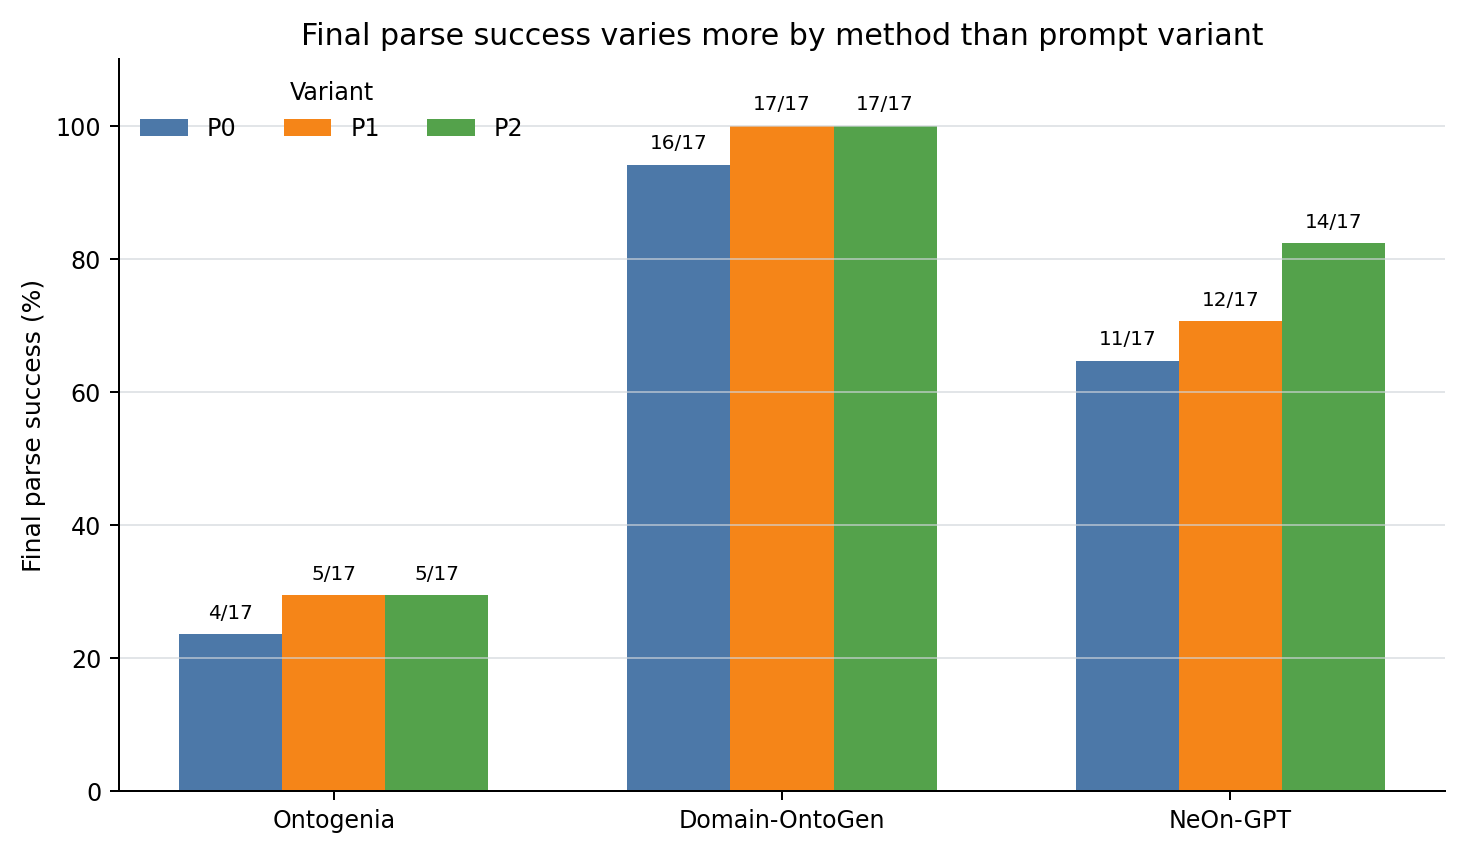
\includegraphics[width=0.82\textwidth]{figures/parse_success_by_method_variant.png}
  \caption{Final parse success by method and prompt variant.}
  \label{fig:parse-success}
\end{figure}

Across all variants, final parse success was 14/51 for Ontogenia, 50/51 for
Domain-OntoGen, and 37/51 for NeOn-GPT. Method-level differences are therefore
much larger than the observed within-method variant differences. Normalization
and syntax repair improve final parseability, particularly for Ontogenia and
NeOn-GPT.

\begin{figure}[H]
  \centering
  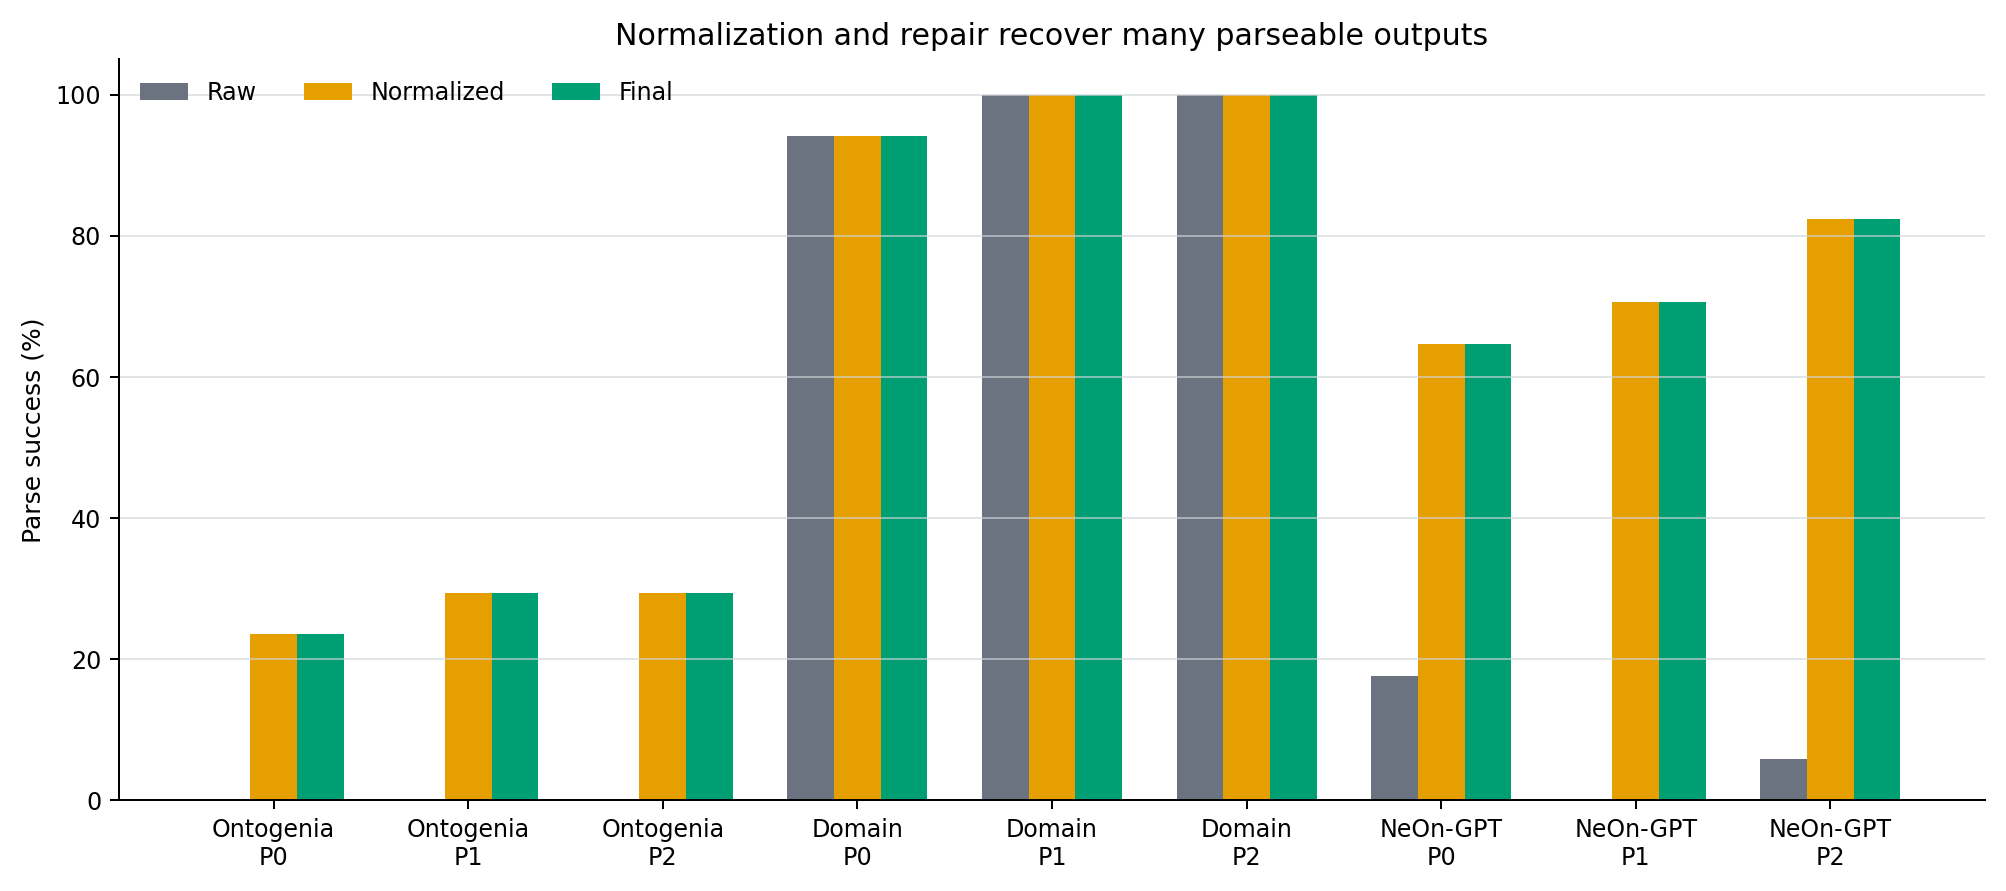
\includegraphics[width=0.84\textwidth]{figures/raw_normalized_final_parse.png}
  \caption{Raw, normalized, and final parse success.}
  \label{fig:parse-stages}
\end{figure}

\subsection{Repairs and length terminations}

The combined experiment records 81 repair calls and 41
\code{done\_reason=length} terminations. Repairs are concentrated in NeOn-GPT.
Length stops also occur in Ontogenia P1/P2 and Domain-OntoGen P0. These events are
retained as evidence rather than silently excluded.

\begin{figure}[H]
  \centering
  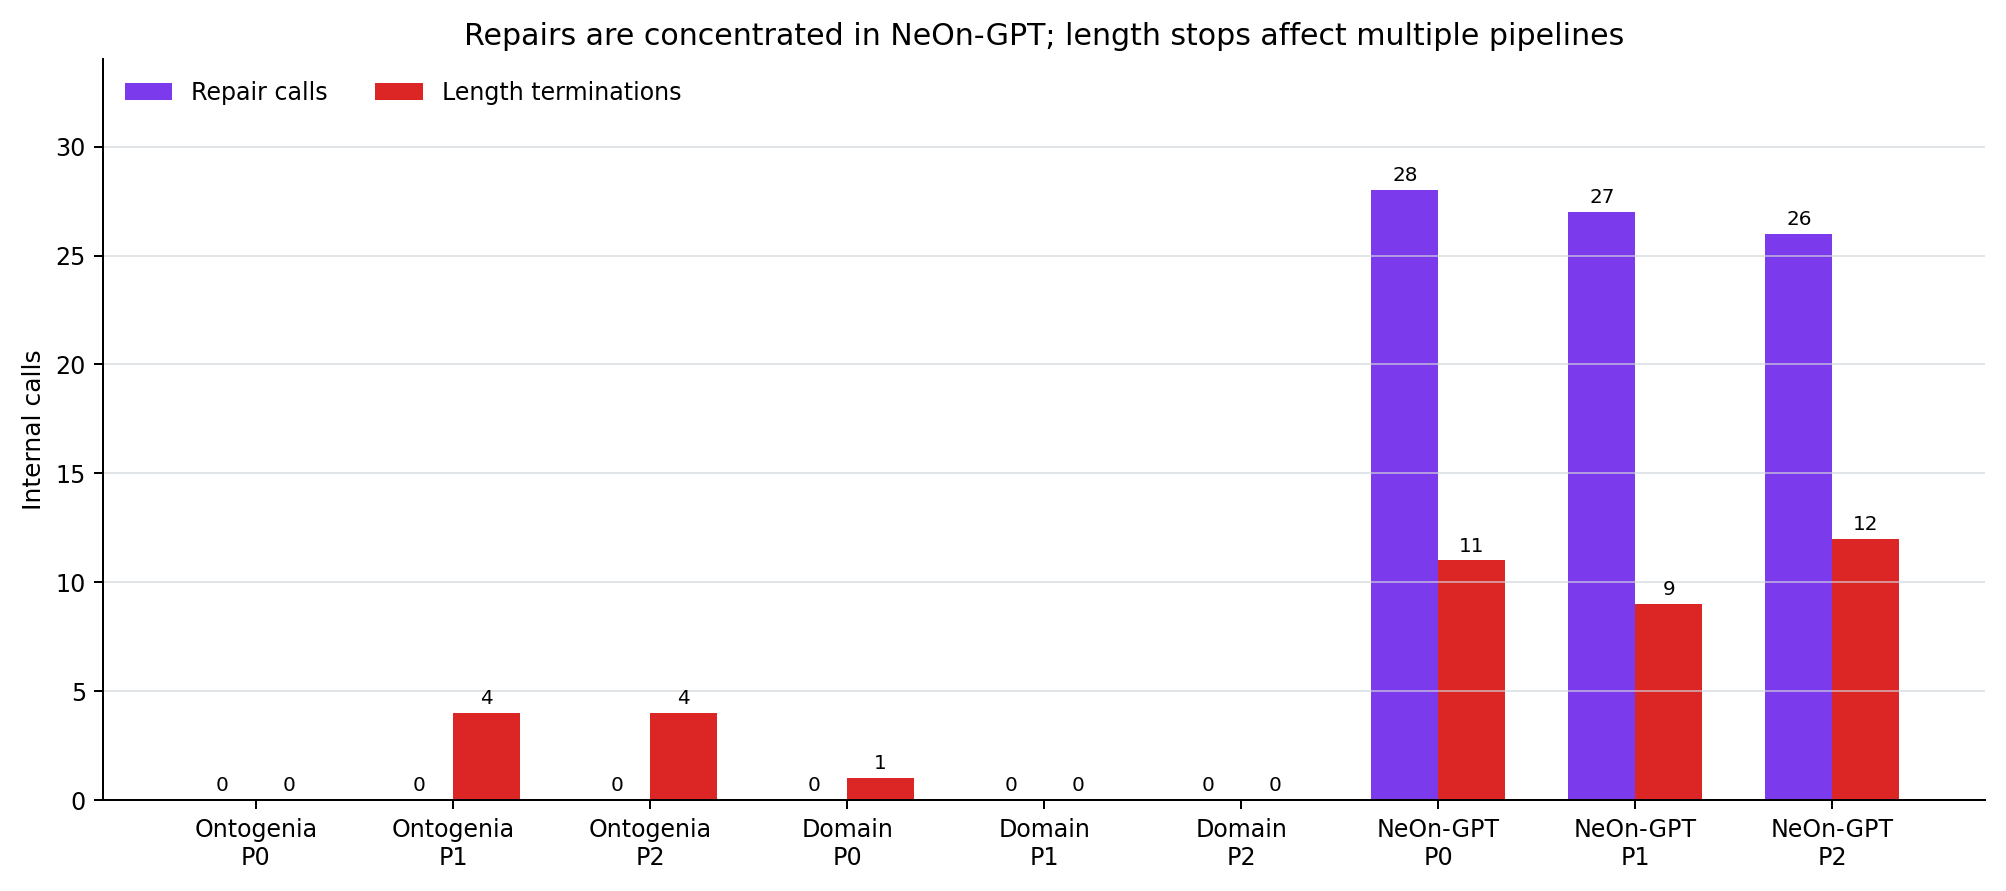
\includegraphics[width=0.82\textwidth]{figures/repair_length_summary.png}
  \caption{Repair calls and length terminations by method and variant.}
  \label{fig:repair-length}
\end{figure}

\subsection{C2 documentation completeness}

C2 is available for 101/153 tasks (66.0\%); the 52 unparseable outputs remain
explicitly unavailable. Across parseable ontologies, class-label coverage is
77.3\% and class-documentation coverage is 43.9\%. Object-property label and
documentation coverage are 85.5\% and 49.1\%, while datatype-property label and
documentation coverage are 68.7\% and 60.7\%. Only one parseable task contains
the required ontology-metadata declaration and descriptive statement.

\begin{figure}[H]
  \centering
  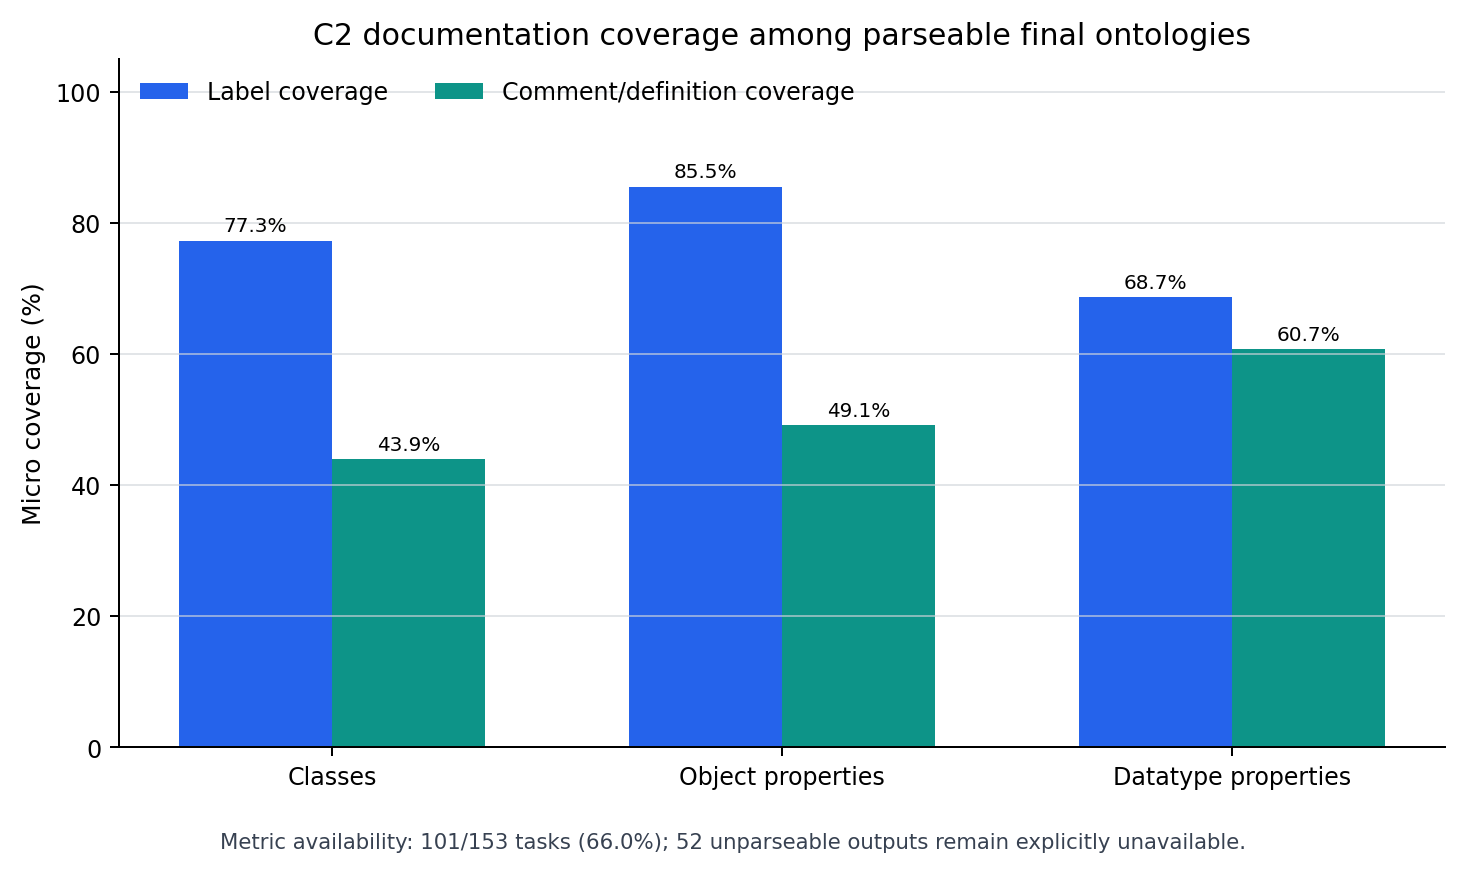
\includegraphics[width=0.90\textwidth]{figures/c2_documentation_coverage.png}
  \caption{Documentation coverage conditional on parseable final ontologies.}
  \label{fig:c2}
\end{figure}

These values are descriptive, not semantic-quality scores. Domain-OntoGen has
very high label coverage but almost no comments or definitions. NeOn-GPT and
parseable Ontogenia outputs often contain richer documentation despite lower
overall parse availability.

\subsection{C3 parse-success inference}

\begin{table}[H]
\centering
\caption{C3 paired statistical summary.}
\label{tab:c3tests}
\small
\begin{tabularx}{\textwidth}{lrrrrX}
\toprule
Method & Triplets & Q p & Term pairs & Wilcoxon p & Interpretation \\
\midrule
Ontogenia & 17 & 0.9048 & 0 & \NA & No significant parse difference; drift comparison not estimable. \\
Domain-OntoGen & 17 & 0.3679 & 16 & 0.3380 & No significant parse difference; P1/P2 drift magnitude not distinguishable. \\
NeOn-GPT & 17 & 0.5292 & 6 & 0.1957 & No significant parse difference; small paired drift sample. \\
\bottomrule
\end{tabularx}
\end{table}

Cochran Q p-values are 0.9048 for Ontogenia, 0.3679 for Domain-OntoGen, and
0.5292 for NeOn-GPT. Every Holm-adjusted McNemar p-value is 1.0. Under the stated
policy, none of the methods shows a statistically significant P0/P1/P2 final
parse-success difference.

\subsection{C3 descriptive term drift}

\begin{table}[H]
\centering
\caption{Term-Jaccard overlap with P0. Lower values indicate more drift.}
\label{tab:jaccard}
\small
\begin{tabular}{llrrrr}
\toprule
Method & Comparison & Eligible n & Median & Min & Max \\
\midrule
Ontogenia      & $J(P0,P1)$ & 0  & \NA    & \NA    & \NA \\
Ontogenia      & $J(P0,P2)$ & 1  & 0.2667 & 0.2667 & 0.2667 \\
Domain-OntoGen & $J(P0,P1)$ & 16 & 0.5682 & 0.3077 & 1.0000 \\
Domain-OntoGen & $J(P0,P2)$ & 16 & 0.6500 & 0.3333 & 1.0000 \\
NeOn-GPT       & $J(P0,P1)$ & 8  & 0.1159 & 0.0000 & 0.4000 \\
NeOn-GPT       & $J(P0,P2)$ & 8  & 0.0000 & 0.0000 & 0.2222 \\
\bottomrule
\end{tabular}
\end{table}

The Domain-OntoGen and especially NeOn-GPT summaries show substantial
descriptive ontology-content drift from P0. Ontogenia has no P0/P1 comparison
and only one P0/P2 value, so no distributional conclusion is justified for that
method. Domain-OntoGen has 16 complete P1/P2 drift pairs (Wilcoxon p=0.3380),
NeOn-GPT has six (p=0.1957), and Ontogenia has none. The NeOn-GPT test uses the
asymptotic Pratt approximation and has low power.

\begin{figure}[H]
  \centering
  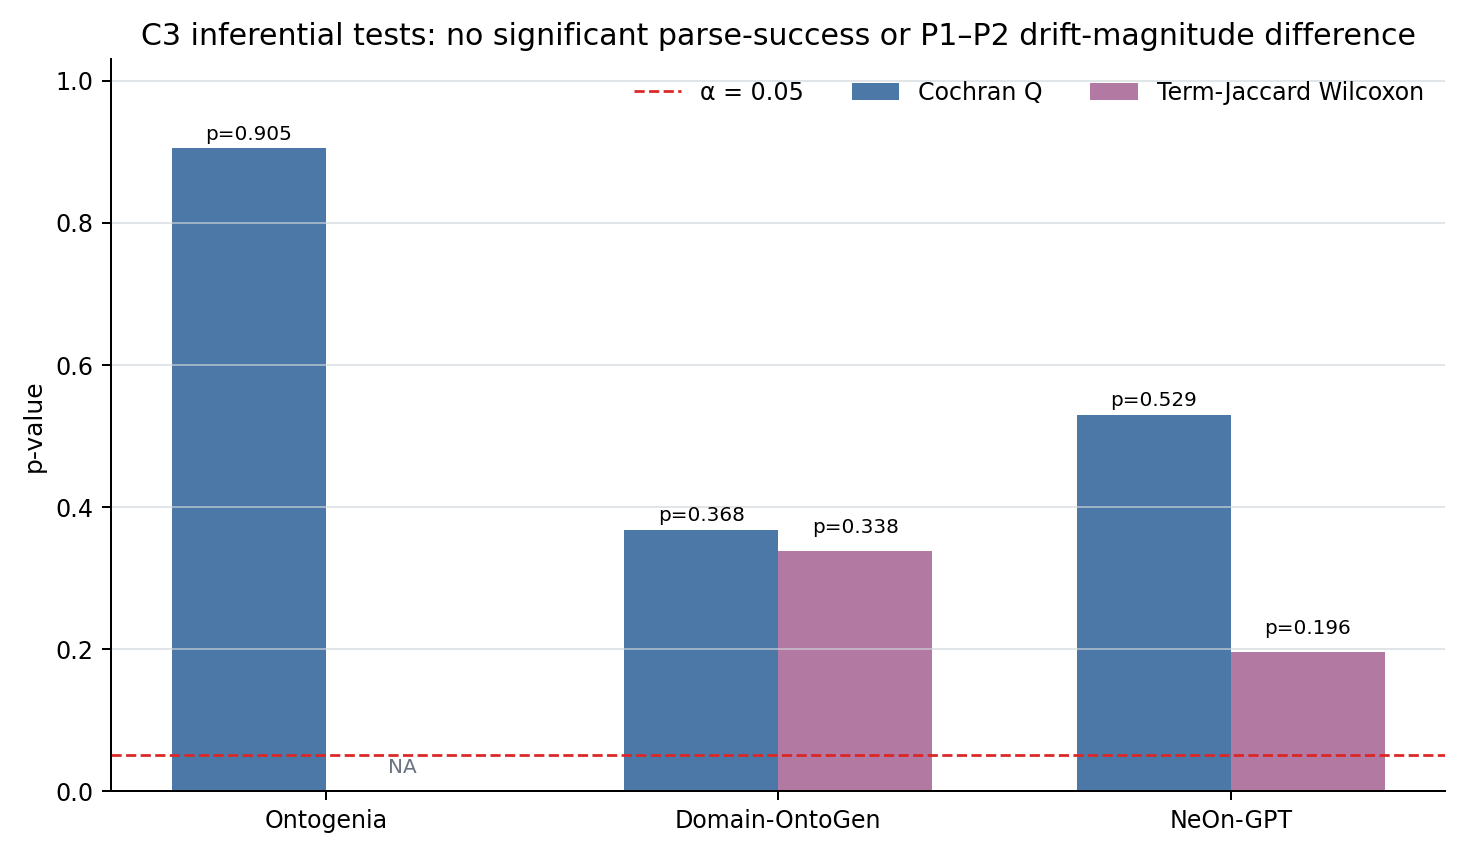
\includegraphics[width=0.90\textwidth]{figures/c3_prompt_sensitivity_summary.png}
  \caption{Prompt-sensitivity summary: parse inference and descriptive term drift.}
  \label{fig:c3}
\end{figure}

Prompt variants did not show statistically significant parse-success
differences, but term overlap still indicates substantial descriptive content
drift. The absence of parse significance is not evidence of prompt invariance or
superiority of P1/P2.

\section{Discussion}

Domain-OntoGen is the most consistently parseable method across all variants,
but its generated ontologies provide little class or property documentation.
NeOn-GPT has intermediate parse robustness and richer documentation, with
additional repair cost and truncation exposure. Ontogenia has the lowest
task-level parse robustness because many CQ fragments contain invalid Turtle.
The Ontogenia failures are associated with invalid generated Turtle rather than
the prompt-assembly code.

P1 and P2 show small descriptive increases in parse success for some cells,
especially NeOn-GPT P2, but the paired tests do not distinguish these changes
from chance under the stated analysis policy. Independently, low term-Jaccard overlap
shows that content can change substantially even when parse-success differences
are not statistically significant. Prompt sensitivity therefore cannot be
reduced to syntax alone.

A repaired ontology can be parseable even when the original response is not.
For this reason, the report presents raw, normalized, and final parse results
separately.

\section{Failure Analysis}

The observed failures fall into three groups:

\begin{enumerate}
  \item \textbf{Model-output quality:} malformed Turtle, incompatible CQ
  fragments, or truncated responses.
  \item \textbf{Post-processing and repair:} normalization and syntax repair
  may recover parseability and are therefore reported separately.
  \item \textbf{Metadata:} the A2 prompt identifier error affected task
  metadata but not the saved request text or response.
\end{enumerate}

\section{Limitations}

\begin{itemize}
  \item Only one local quantized model, one seed, and one context/output budget
  were evaluated.
  \item The dataset contains 17 scenarios; some paired term denominators are
  small or zero.
  \item Parse success does not establish conceptual correctness, CQ coverage,
  logical consistency, or practical ontology usefulness.
  \item C2 is conditional on syntactically parseable output and does not judge
  semantic quality of documentation.
  \item Normalization and repair affect observed final parseability.
  \item The A2 metadata error required verification from the saved request text.
  \item Public source ontologies may create contamination risk; the current work
  does not claim to eliminate that risk.
\end{itemize}

\section{Reproducibility and Submission Artifacts}

The full research workspace retains the dataset, prompts, model settings,
requests, responses, parse stages, and telemetry. The repository includes the
implementation, final tables, statistical outputs, and one complete A2 P1
example. The full A1/A2 output trees are stored separately because of their
size.

Key submitted artifacts include:

\begin{itemize}
  \item \code{restapi/}: provider, adapter, API, metrics, and artifact logic;
  \item \code{scripts/}: preparation, execution, and analysis tools;
  \item \code{datasets/ontology\_generation/}: normalized data and prompts;
  \item \code{config/}: experiment and statistical settings;
  \item \code{results/final\_c2\_c3\_summary.csv}: final method-level results;
  \item \code{evidence/}: one complete A2 P1 request example;
\end{itemize}

Re-running model generation requires the same Ollama model and constitutes a
new execution. The existing results can be inspected without a live model. The repository implementation is based on and
extends the Bench4KE project \cite{bench4ke_repository}.

\section{Conclusion}

The project satisfies the course scope by implementing mandatory local Ollama
support and two additional evaluation components, then applying the three
required ontology-generation methods to the 17-item executable dataset.

Domain-OntoGen achieved the highest parse robustness, NeOn-GPT combined
intermediate parseability with richer documentation and higher repair exposure,
and Ontogenia remained the least robust at task-level Turtle parsing. P0/P1/P2
did not differ significantly in paired parse-success tests. However, descriptive
term-Jaccard overlap showed substantial content drift, especially for NeOn-GPT,
so non-significance does not establish prompt invariance.

The implementation provides a practical basis for comparing local models,
prompt variants, and ontology-generation methods in future experiments.

\clearpage
\appendix

\section{Detailed Parse Summary}

\begin{table}[H]
\centering
\caption{Raw, normalized, and final parse counts.}
\small
\begin{tabular}{llrrrr}
\toprule
Method & Variant & Tasks & Raw & Normalized & Final \\
\midrule
Ontogenia & P0 & 17 & 0 & 4 & 4 \\
Ontogenia & P1 & 17 & 0 & 5 & 5 \\
Ontogenia & P2 & 17 & 0 & 5 & 5 \\
Domain-OntoGen & P0 & 17 & 16 & 16 & 16 \\
Domain-OntoGen & P1 & 17 & 17 & 17 & 17 \\
Domain-OntoGen & P2 & 17 & 17 & 17 & 17 \\
NeOn-GPT & P0 & 17 & 3 & 11 & 11 \\
NeOn-GPT & P1 & 17 & 0 & 12 & 12 \\
NeOn-GPT & P2 & 17 & 1 & 14 & 14 \\
\bottomrule
\end{tabular}
\end{table}

\section{Generation Cost and Runtime Summary}

{\scriptsize
\setlength{\tabcolsep}{3pt}
\begin{longtable}{llrrrrr}
\caption{Internal-call telemetry by method and variant.}\\
\toprule
Method & Variant & Calls & Prompt tokens & Completion tokens & Total tokens & Seconds \\
\midrule
\endfirsthead
\toprule
Method & Variant & Calls & Prompt tokens & Completion tokens & Total tokens & Seconds \\
\midrule
\endhead
Ontogenia & P0 & 74 & 160,584 & 110,780 & 271,364 & 532.761 \\
Ontogenia & P1 & 74 & 163,322 & 122,812 & 286,134 & 594.151 \\
Ontogenia & P2 & 74 & 166,282 & 136,927 & 303,209 & 651.114 \\
Domain-OntoGen & P0 & 74 & 169,142 & 70,871 & 240,013 & 337.428 \\
Domain-OntoGen & P1 & 74 & 171,954 & 49,234 & 221,188 & 249.039 \\
Domain-OntoGen & P2 & 74 & 174,914 & 55,740 & 230,654 & 268.731 \\
NeOn-GPT & P0 & 45 & 165,240 & 226,560 & 391,800 & 540.968 \\
NeOn-GPT & P1 & 44 & 149,032 & 196,769 & 345,801 & 528.101 \\
NeOn-GPT & P2 & 43 & 146,715 & 197,692 & 344,407 & 760.189 \\
\midrule
\textbf{Total} & \textbf{All} & \textbf{576} & \textbf{1,467,185} & \textbf{1,167,385} & \textbf{2,634,570} & \textbf{4,462.483} \\
\bottomrule
\end{longtable}
}

\bibliographystyle{plain}
\bibliography{references}

\end{document}
